\documentclass{article}
\usepackage{graphicx} % Para incluir imágenes
\usepackage[spanish]{babel}
\usepackage{makeidx}
\usepackage{geometry}
\usepackage{amsmath}
\usepackage{graphicx}
\usepackage{caption}
\usepackage{pdfpages}
\usepackage{hyperref}
\usepackage{placeins}
\hypersetup{
    colorlinks,
    citecolor=black,
    filecolor=black,
    linkcolor=black,
    urlcolor=black
}



\geometry{a4paper, total={170mm,257mm}, left=20mm, top=20mm}
\renewcommand{\familydefault}{\sfdefault}


\begin{document}
\begin{titlepage}
    \centering
    \Large
    Universidad Central de Venezuela\\
    Facultad de Ingeniería\\
    Escuela de Ingeniería Eléctrica
    \vspace*{8cm}

    \Huge
    \textbf{Prelaboratorio N° 11: } 

    \textbf{Multivibradores}
    \vfill


    \Large

    Emerson Warhman \\
    C.I. 25.795.480 \\
    \today

\end{titlepage}
\tableofcontents
\newpage

\section{Introducción}

% \section{Introducción}

En el ámbito de la electrónica, los amplificadores operacionales son componentes fundamentales que se utilizan en una amplia variedad de aplicaciones, desde sistemas de audio hasta equipos de medición y control. Un amplificador operacional es un dispositivo de alta ganancia con dos entradas y una salida, que puede amplificar señales de voltaje muy pequeñas.

El objetivo de este informe de laboratorio es analizar el comportamiento y las características de un amplificador operacional en sus etapas diferencial, impulsora y de potencia y del circuito multietapas en diferentes conilustraciónciones. Se realizarán mediciones de los puntos estáticos, modelos dinámicos, ganancia respuesta en frecuencia y utilizando circuitos con realimentación negativa y positiva.  


\section{Resumen}

% \subsection{Filtros activos}

Un filtro es en general aquel dispositivo que modifica linealmente el
contenido espectral de una señal. Un filtro activo es aquel el cual, ademas de contar con elementos pasivos, también tiene elementos activos cómo el amplificador operacional.

No es difícil encontrar una situación cuyos requerimientos exijan un filtro de orden alto y tampoco es imposible realizarlo, lo difícil es sintonizarlo, esto es, hacer que cada coeficiente de la función de transferencia tome el valor adecuado para cumplir con los requerimientos.

La sintonización se hace difícil, porque los parámetros de red susceptibles de variarse, modifican a mas de un coeficiente a la vez y si el número de coeficientes es alto, la tarea, además de ser iterativa, es muy costosa en tiempo y en equipos.

Si el orden del filtro es alto, entonces puede dividirse en una cascada de etapas de 2do orden y a lo mas una de primer orden en el caso de orden impar

\begin{align*}
    H &= \frac{1}{s^5 + 3.236s^4 + 5.236s^3 + 5.236s^2 + 3.236s + 1} \\
    H &= \frac{1}{(s^2 + 0.61803s + 1) \cdot (s^2 + 1.61803) \cdot (s + 1)}
\end{align*}

De manera tal que solo sea necesario sintonizar varias etapas de 2do orden y quizás de 1er orden, que aunque para cada una de ellas debe sintonizarse iterativamente, llevarán mucho menor tiempo y con la garantía de convergencia.

\subsubsection{Función de transferencia de los filtros}

Las funciones de transferencia de los filtros más utilizados son bien conocidas y son las siguientes:

\begin{itemize}
\item 
Pasa bajos:
\begin{multicols}{2}
\begin{equation}
    H(s) = \frac{H_o \cdot \omega_o^2}{s^2 + \alpha \cdot \omega_o \cdot s + \omega_o^2}
    \label{eq:func-transferencia-pasa-bajos}
\end{equation}
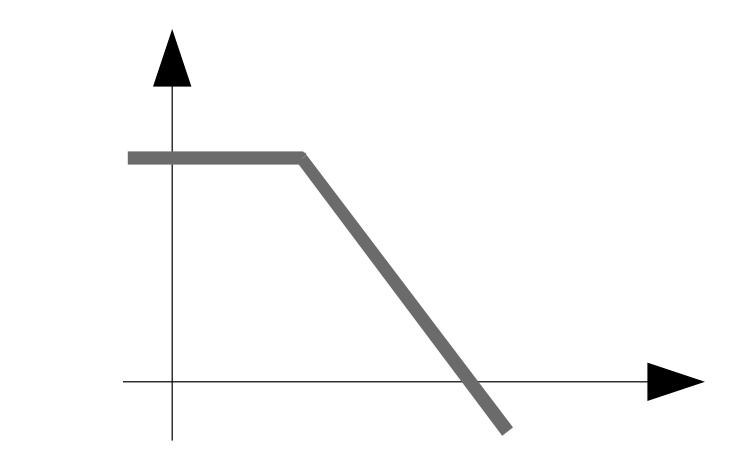
\includegraphics[width=0.1\textwidth]{marco-teorico/respuesta-freq-pasa-bajos.png}
\end{multicols}
    \item 
    Pasa banda:
    \begin{multicols}{2}
    \begin{equation}
        H(s) = \frac{H_o \cdot \omega_o \cdot s}{s^2 + \alpha \cdot \omega_o \cdot s + \omega_o^2}
        \label{eq:func-transferencia-pasa-banda}
    \end{equation}
    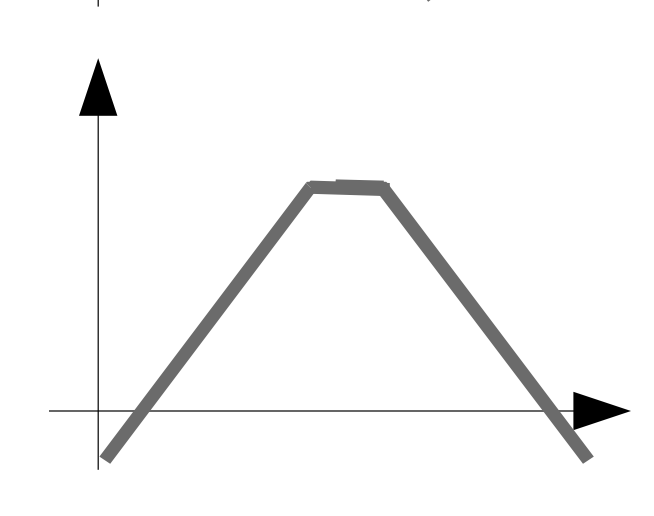
\includegraphics[width=0.1\textwidth]{marco-teorico/respuesta-freq-pasa-banda.png}
    \end{multicols}
Pasa altos:
\begin{multicols}{2}
\begin{equation}
    H(s) = \frac{H_o \cdot s^2}{s^2 + \alpha \cdot \omega_o \cdot s + \omega_o^2}
    \label{eq:func-transferencia-pasa-altos}
\end{equation}
    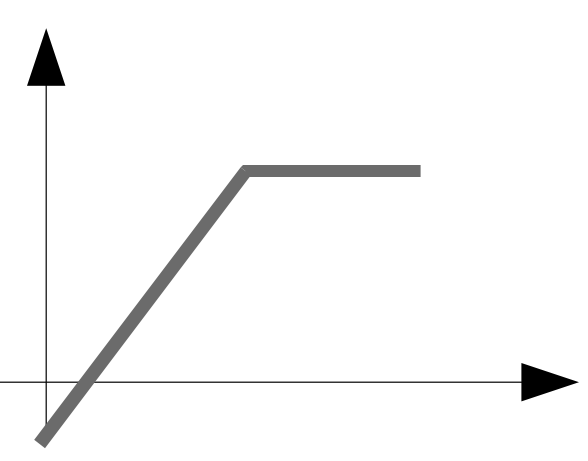
\includegraphics[width=0.1\textwidth]{marco-teorico/respuesta-freq-pasa-altos.png}
\end{multicols}
Rechaza banda:
\begin{multicols}{2}
\begin{equation}
    H(s) = \frac{H_o \left( s^2 + \omega_o^2 \right)}{s^2 + \alpha \cdot \omega_o \cdot s + \omega_o^2}
    \label{eq:func-transferencia-rechaza-banda}
\end{equation}
    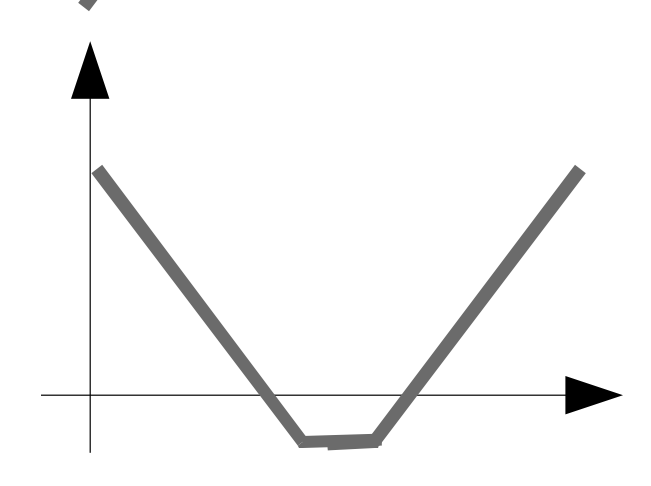
\includegraphics[width=0.1\textwidth]{marco-teorico/respuesta-freq-rechaza-banda.png}
\end{multicols}
\end{itemize}

\subsection{Filtros de múltiples realimentaciones}

Esta topología puede convertirse en un cualquiera de las funciones de segundo orden (pasa bajo, pasa alto o pasa banda) con solo ubicar apropiadamente resistencias y condensadores.

\begin{figure}[ht]
    \centering
    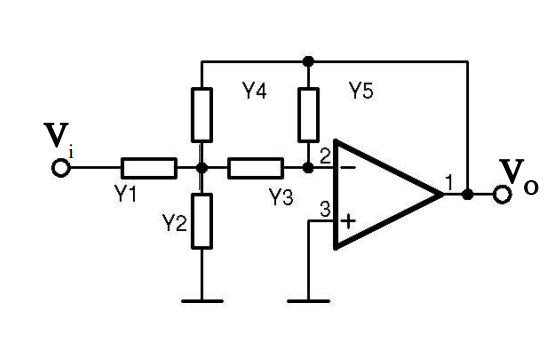
\includegraphics[width=0.5\textwidth]{marco-teorico/filtro-multiples-realimentaciones.png}
    \caption{Filtro de múltiples realimentaciones}
    \label{fig:filtro-multiples-realimentacion}
\end{figure}

La función de transferencia puede resolverse de varias maneras, pero resulta compacto en términos de sus admitancias y usando el inversor $-Y_3/Y_5$ como amplificador base.

Utilizando el método del amplificador desvanecido, tenemos:

$$A_b = - \frac{Y_3}{Y_5}$$

\begin{align*}
    a_{io} &= 0 \\
    a_{i1} &= \frac{Y_1}{Y_1 + Y_2 + Y_3 + Y_4}\\
    a_{31} &= \frac{Y_4}{Y_1 + Y_2 + Y_3 + Y_4}\\
    a_{3o} &= 1
\end{align*}

Aplicandolo a la formula MAD:

\begin{equation}
    \frac{V_o}{V_i} = \frac{Y_1}{Y_1 + Y_2 + Y_3 + Y_4} \frac{\frac{-Y_3}{Y_5}}{1 - \frac{Y_4}{Y_1 + Y_2 + Y_3 + Y_4} \WrapParenthesis{\frac{-Y_3}{Y_5}}}
\end{equation}

lo cual queda como:

\begin{equation}
    \frac{V_o}{V_i} = \frac{-Y_1 \cdot Y_3}{Y_5(Y_1 + Y_2 + Y_3 + Y_4)+ Y_3.Y_4} 
    \label{eq:filtro-multirealimentacion}
\end{equation}

\subsubsection{Filtro pasa bajo de múltiples realimentaciones}

\begin{figure}[ht]
    \centering
    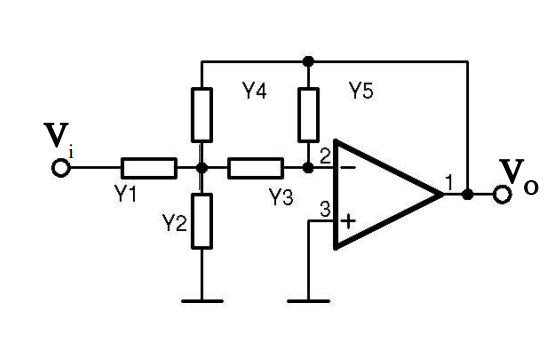
\includegraphics[width=0.5\textwidth]{marco-teorico/filtro-multiples-realimentaciones.png}
    \caption{Filtro pasa bajo de múltiples realimentaciones}
    \label{fig:filtro-multiples-realimentacion-pasa-bajo}
\end{figure}

Al sustituir las admitancias $Y_2$ y $Y_5$ de la figura \ref{fig:filtro-multiples-realimentacion} por condensadores, obtenemos un filtro pasa bajo con la siguiente función de transferencia:

\begin{equation}[ht]
    H(s) = \frac{V_o(s)}{V_i(s)} = \frac{-\frac{1}{R_1}\cdot R_2C_2 C_5}{s^2 + (1/C_2)(1/R_1 + 1/R_3 + 1/R_4)s + 1/(R_3 R_4 C_2 C_5)}
    \label{eq:func-transferencia-pasa-bajos-multirealimentacion}
\end{equation}

\subsection{Filtro por fuente de tensión controlada por tensión o Sallen-Key}

Usando esta estructura y ubicando en ella solo capacitancias y resistencias (sin inductancias) pueden lograrse los tres tipos de filtro básicos, esta vez, sin inversión de fase.

\begin{figure}[ht]
    \centering
    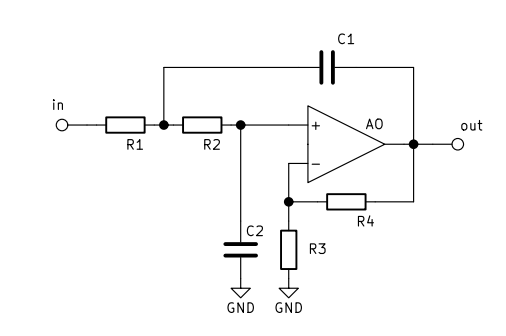
\includegraphics[width=0.5\textwidth]{marco-teorico/filtro-sallen-key.png}
    \caption{Filtro con topología de Sallen-Key}
    \label{fig:filtro-activo-sallen-key}
\end{figure}

Tomando en cuenta que:

\begin{equation}
    K = 1 + \frac{R_B}{R_A}
\end{equation}

Aplicando el método del amplificador desvanecido, tenemos:

\begin{align}
    A &= K \\
    a_{io} &= 0 \\
    a_{i1} &= \frac{Y_1}{Y_1 + Y_2 + Y_3 + \WrapParenthesis{\frac{Y_4 Y_5}{Y_4}} + Y_5} \WrapParenthesis{\frac{Y_4}{Y_4 + Y_5}} \\
    a_{30} &= 1 \\
    a_{31} &= \frac{Y_2}{Y_1 + Y_2 + Y_3 + \WrapParenthesis{\frac{Y_4 Y_5}{Y_4 + Y_5}}} \WrapParenthesis{\frac{Y_4}{Y_4 + Y_5}} \\
\end{align}

Sustituyendo en la ecuación MAD:

\begin{equation}
    H(s) = \frac{V_o}{V_i} = \frac{Y_1 Y_4 K}{(Y_1 + Y_2 * Y_3 + Y_4)Y_5 + (Y_1 +Y_2(1-K)+Y_3)Y_4}
\end{equation}

\subsubsection{Filtro pasa bajo de topología de Sallen-Key}

sustituyendo $Y_2$ y $Y_5$ por condensadores, obtenemos un filtro pasa bajo con la siguiente función de transferencia:


\begin{figure}
    \centering
    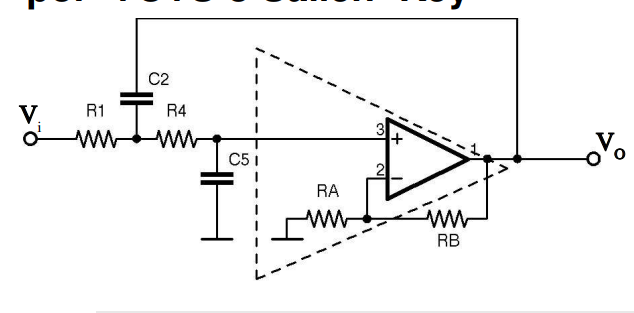
\includegraphics[width=0.5\textwidth]{marco-teorico/filtro-pasa-bajo-sallen-key.png}
    \caption{Filtro pasa bajo de topología de Sallen-Key}
\end{figure}

Al sustituir las admitancias $Y_2$ y $Y_5$ de la figura \ref{fig:filtro-activo-sallen-key} por condensadores, obtenemos un filtro pasa bajo con la siguiente función de transferencia:

\begin{equation}
    H(s) = \frac{\frac{K}{R_1 R_4 C_2 C_5}}{s^2 + \left(\frac{1}{R_1 C_2} + \frac{1}{R_4 C_2} + \left(1 - K\right) \frac{1}{R_4 C_5}\right)s + \frac{1}{R_1 R_4 C_2 C_5}}
    \label{eq:transferencia-pasa-bajo-sallen-key}
\end{equation}

% \include{src/metodologia/metodología.tex}


\subsubsection{Tensión de offset}

El cuadro \ref{tab:resultados-tension-offset} muestra las mediciones de tensión de offset.

\begin{table}[h!]
\centering
\begin{tabular}{|c|c|c|c|c|c|c|c|}
\hline
$V_o$ [V] & $\Delta V_o$ [V] & $R_f$ [K$\Omega$] & $\Delta R_f$ [K$\Omega$] & $R_s$ [$\Omega$] & $\Delta R_s$ [$\Omega$] & $V_{os}$ [mV] & $\Delta V_{os}$ [mV] \\ \hline
-8 & 0.4 & 100.000 & 5.000 & 100 & 5 & -8.000 & 0.690 \\ \hline
\end{tabular}
\caption{Mediciones de tensión de offset.}
\label{tab:resultados-tension-offset}
\end{table}

\subsubsection{Corriente de polarización Bias}

El cuadro \ref{tab:resultados-corriente-polarizacion} muestra las mediciones de las corrientes de polarización.

\begin{table}[h!]
\centering
\resizebox{\textwidth}{!}{  % Escala la tabla al ancho del texto
\begin{tabular}{|c|c|c|c|c|c|c|c|c|c|c|c|}
\hline
$V_o$ [V] & $\Delta V_o$ [V] & $R_f$ [$k\Omega$] & $\Delta R_f$ [$k\Omega$] & $R_s$ [$\Omega$] & $\Delta R_s$ [$\Omega$] & $R_b$ [$M\Omega$] & $\Delta R_b$ [$M\Omega$] & $V_{os}$ [mV] & $\Delta V_{os}$ [mV] & $I_B$ [nA] & $\Delta I_B$ [nA] \\ \hline
-8 & 0.4 & 100 & 5 & 100 & 5 & 22 & 1.1 & -8.000 & 0.690 & -0.00069 & 0.045 \\ \hline
8 & 1 & 100 & 5 & 100 & 5 & 22 & 1.1 & -8.000 & 0.690 & 0.73 & 0.071 \\ \hline
\end{tabular}
}
\caption{Mediciones de corriente de polarización.}
\label{tab:resultados-corriente-polarizacion}
\end{table}

El cuadro \ref{tab:resultados-corrientes-bias} muestra las mediciones de las corrientes $I_{B1}$, $I_{B2}$ e $I_{BIAS}$.

\begin{table}[h!]
\centering
\begin{tabular}{|c|c|c|c|c|c|}
\hline
$I_{B1}$ [nA] & $\Delta I_{B1}$ [nA] & $I_{B2}$ [nA] & $\Delta I_{B2}$ [nA] & $I_{BIAS}$ [nA] & $\Delta I_{BIAS}$ [nA] \\ \hline
-0.00069 & 0.045 & 0.73 & 0.071 & -0.73 & 0.084 \\ \hline
\end{tabular}
\caption{Mediciones de corrientes $I_{B1}$, $I_{B2}$ e $I_{BIAS}$.}
\label{tab:resultados-corrientes-bias}
\end{table}

\subsubsection{Mediciones del GBWP}

\begin{table}[h!]
\centering
\resizebox{\textwidth}{!}{
\begin{tabular}{|c|c|c|c|c|c|c|c|}
\hline
A & $\Delta$A & $f_l$ [Hz] & $\Delta f_l$ [Hz] & $f_h$ [kHz] & $\Delta f_h [kHz] $ & GBWP & $\Delta$GBWP [Hz] \\ \hline
100 & 7.86 & 2 & 0.8 & 7.14 & 0.051 & 714085.71 & 56335.44 \\ \hline
11.11 & 0.83 & 2 & 0.08 & 75.76 & 2.30 & 841728.62 & 67887.11 \\ \hline
1.00 & 0.08 & 2 & 0.08 & 892.86 & 31.89 & 892855.14 & 77056.50 \\ \hline
\end{tabular}
}
\caption{Mediciones del producto ganancia ancho de banda.}
\label{tab:resultados-gbwp}
\end{table}

\subsubsection{Mediciones del Slew Rate}

la figura \ref{fig:resultados-slew-rate} muestra la medición de la forma de onda del slew rate.

\begin{figure}[h!]
\centering
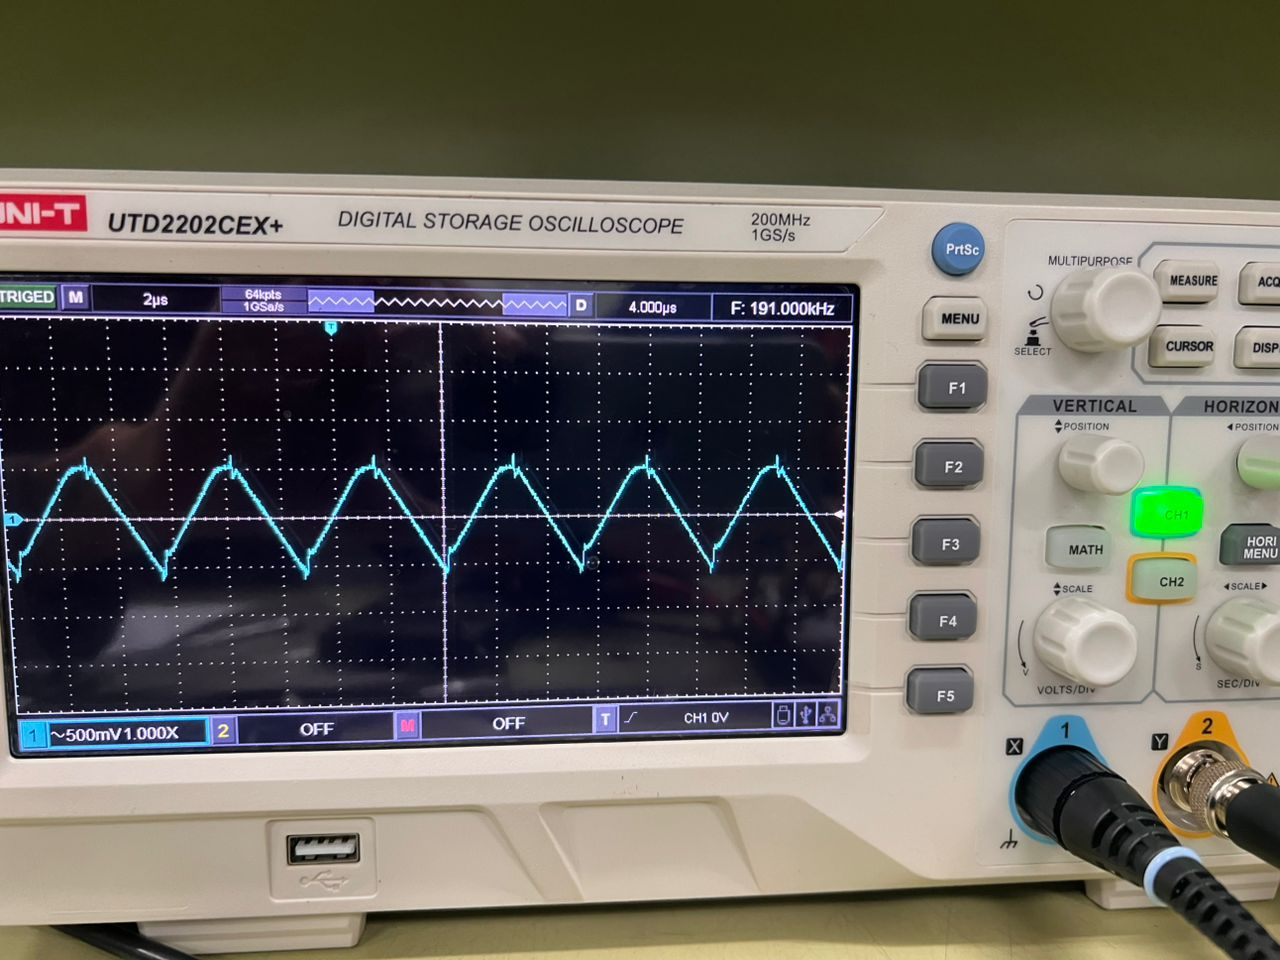
\includegraphics[width=0.5\textwidth]{resultados/slewrate.jpg}
\caption{Mediciones del slew rate.}
\label{fig:resultados-slew-rate}
\end{figure}

El cuadro \ref{tab:resultados-slew-rate} muestra las mediciones del slew rate.

\begin{table}[h!]
\centering
\begin{tabular}{|c|c|c|c|c|c|}
\hline
$V_o$ [V] & $\Delta V_o$ [V] & $\Delta t$ [$\mu$s] & $\Delta(\Delta t)$ [$\mu$s] & SR [V/$\mu$s] & $\Delta$SR [V/$\mu$s] \\ \hline
1 & 0.1 & 2 & 0.4 & 0.500 & 0.112 \\ \hline
\end{tabular}
\caption{Mediciones del slew rate.}
\label{tab:resultados-slew-rate}
\end{table}


\subsubsection{Mediciones de la corriente de cortocircuito}

\begin{table}[h!]
\centering
\begin{tabular}{|c|c|c|c|c|c|}
\hline
V [V] & $\Delta$V [V] & R [k$\Omega$] & $\Delta$R [k$\Omega$] & $I_{SC}$ [mA] & $\Delta I_{SC}$ [mA] \\ \hline
2.0 & 0.2 & 6.800 & 0.034 & 294.12 & 29.45 \\ \hline
\end{tabular}
\caption{Mediciones de la corriente de cortocircuito.}
\label{tab:resultados-corriente-cortocircuito}
\end{table}

El cuadro \ref{tab:resultados-corriente-cortocircuito} muestra las mediciones de la corriente de cortocircuito.







\section{Análisis de resultados}

\section{Conclusiones}

\section{Anexos}
% 
\begin{figure}[ht]
    \centering
    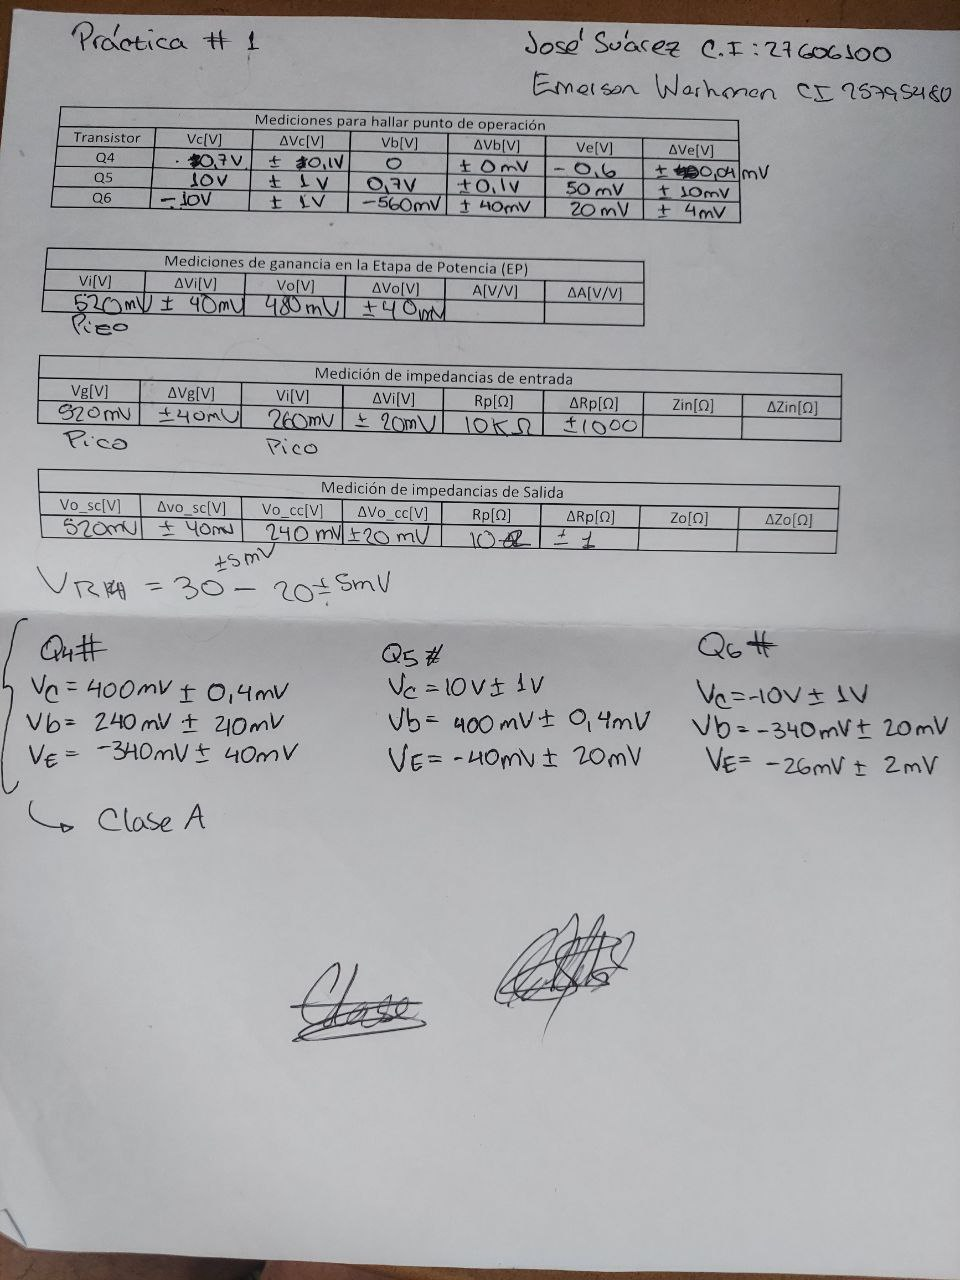
\includegraphics[width=1.0\textwidth]{src/images/p1/p1-hoja-de-datos.jpg}
    \caption{Hoja de datos práctica N° 1}
    \label{fig:hoja-de-datos-p1}
\end{figure}

\begin{figure}[ht]
    \centering
    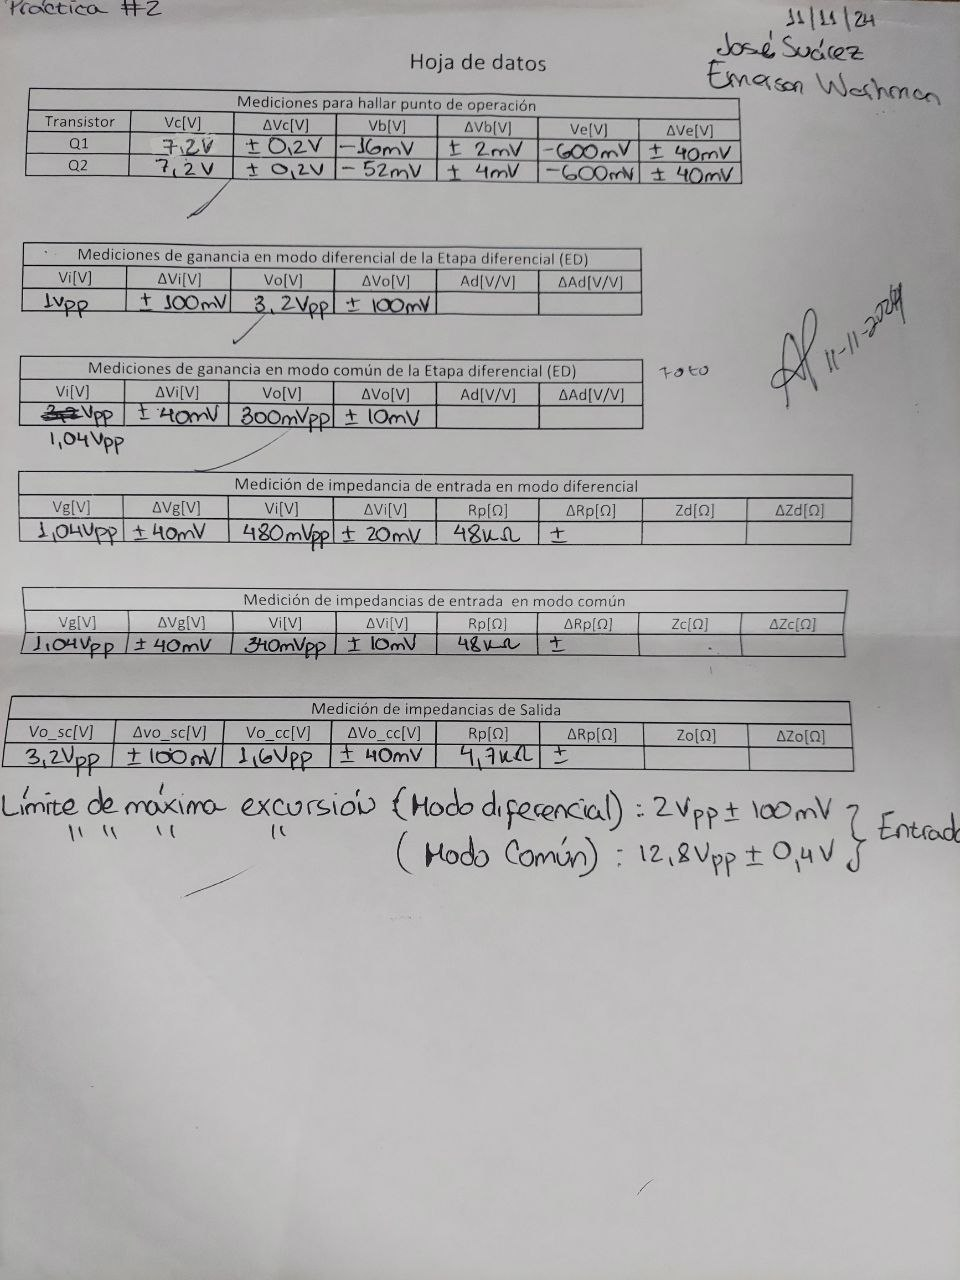
\includegraphics[width=1.0\textwidth]{src/images/p2/p2-hoja-de-datos.jpg}
    \caption{Hoja de datos práctica N° 2}
    \label{fig:hoja-de-datos-p2}
\end{figure}

\begin{figure}[ht]
    \centering
    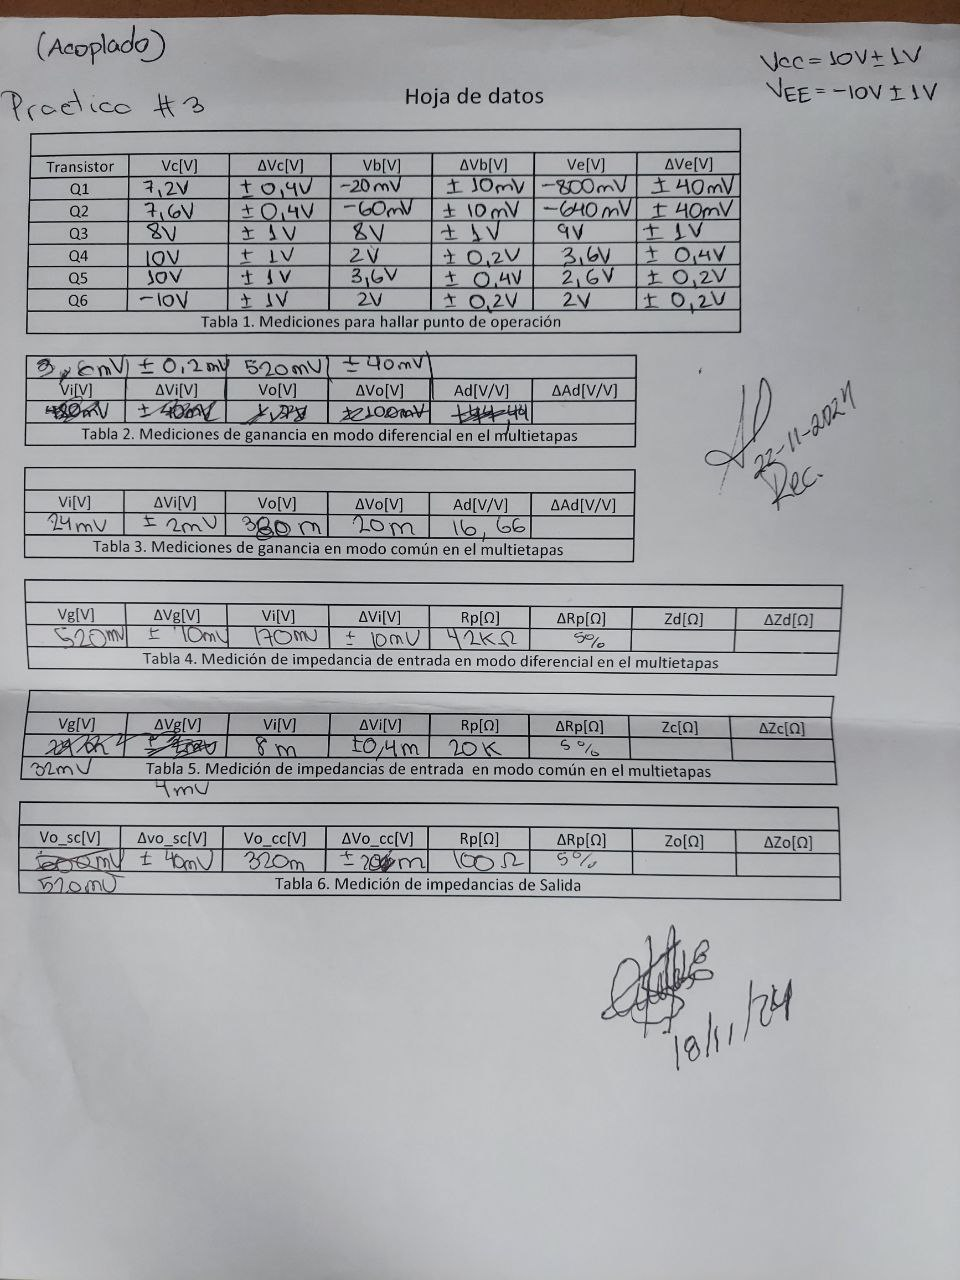
\includegraphics[width=1.0\textwidth]{src/images/p3/p3-hoja-de-datos.jpg}
    \caption{Hoja de datos práctica N° 3-1}
    \label{fig:hoja-de-datos-p3-1}
\end{figure}

\begin{figure}[ht]
    \centering
    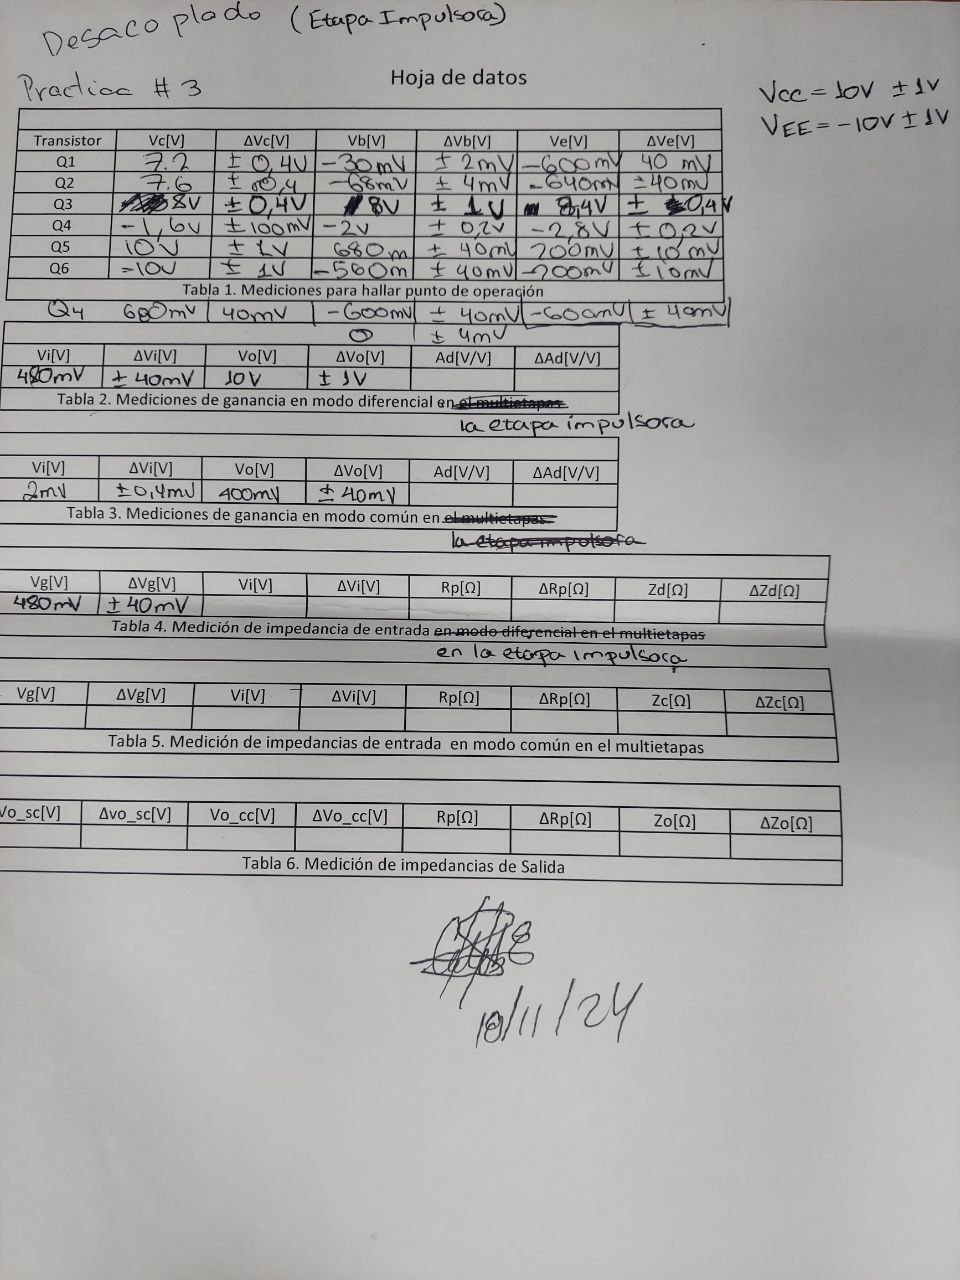
\includegraphics[width=1.0\textwidth]{src/images/p3/p3-hoja-de-datos-2.jpg}
    \caption{Hoja de datos práctica N° 3-2}
    \label{fig:hoja-de-datos-p3-2}
\end{figure}

\begin{figure}[ht]
    \centering
    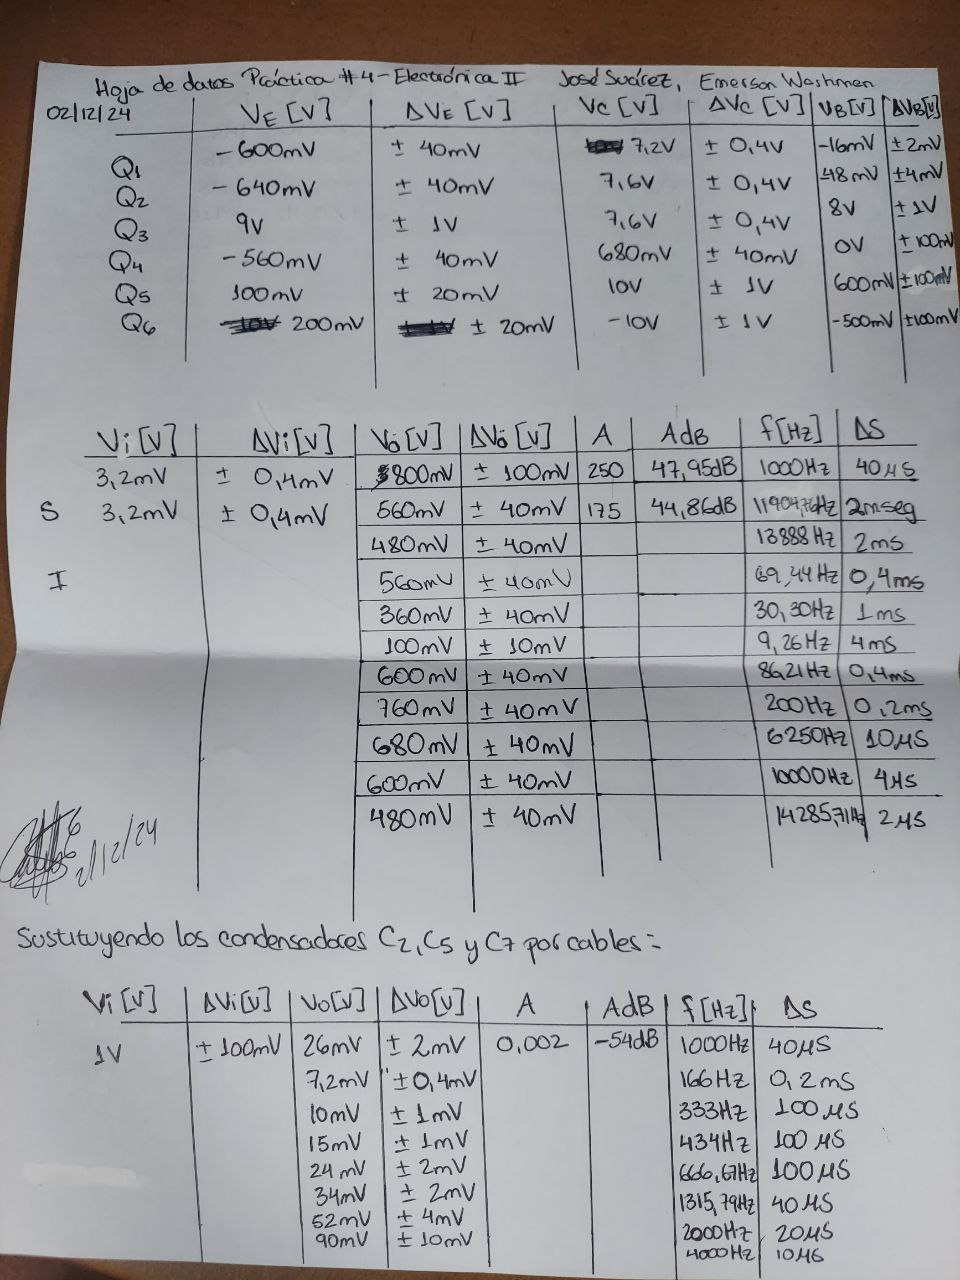
\includegraphics[width=1.0\textwidth]{src/images/p4/p4-hoja-de-datos-1.jpg}
    \caption{Hoja de datos práctica N° 4-1}
    \label{fig:hoja-de-datos-p4-1}
\end{figure}

\begin{figure}[ht]
    \centering
    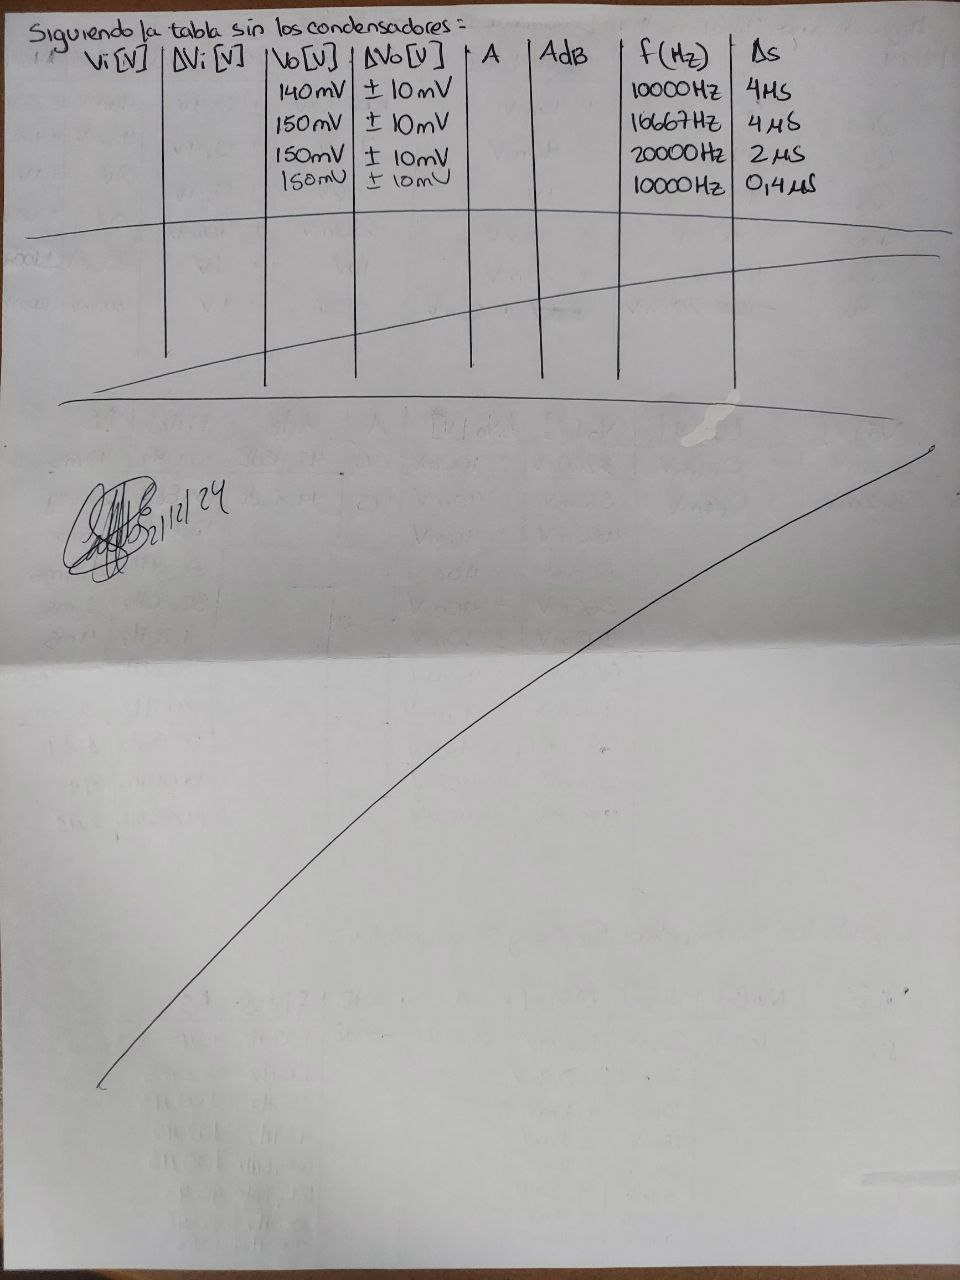
\includegraphics[width=1.0\textwidth]{src/images/p4/p4-hoja-de-datos-2.jpg}
    \caption{Hoja de datos práctica N° 4-2}
    \label{fig:hoja-de-datos-p4-2}
\end{figure}

\begin{figure}[ht]
    \centering
    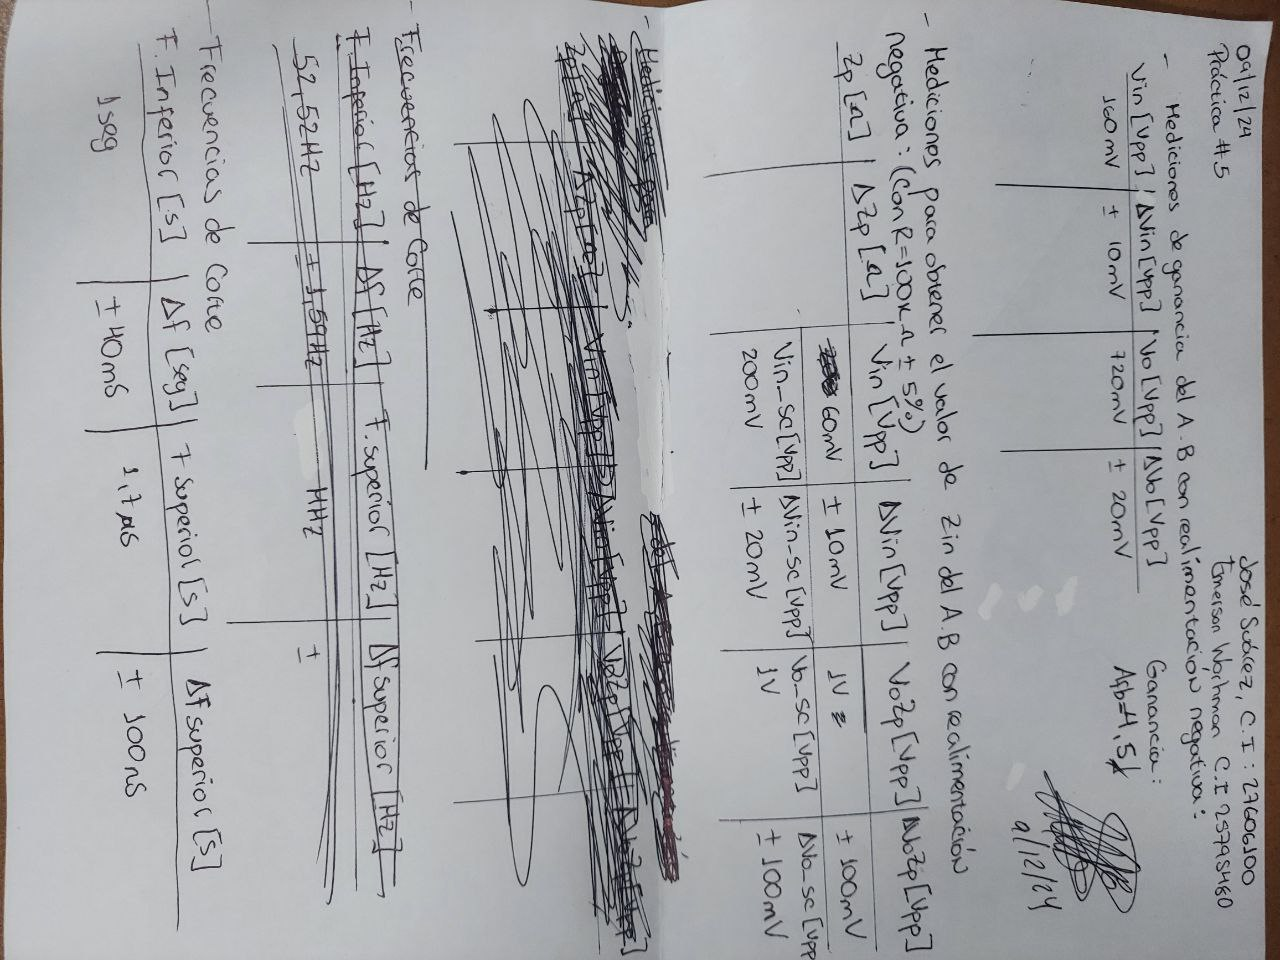
\includegraphics[width=1.0\textwidth, angle=90]{src/images/p5/p5-hoja-de-datos-1.jpg}
    \caption{Hoja de datos práctica N° 5-1}
    \label{fig:hoja-de-datos-p5-1}
\end{figure}

\begin{figure}[ht]
    \centering
    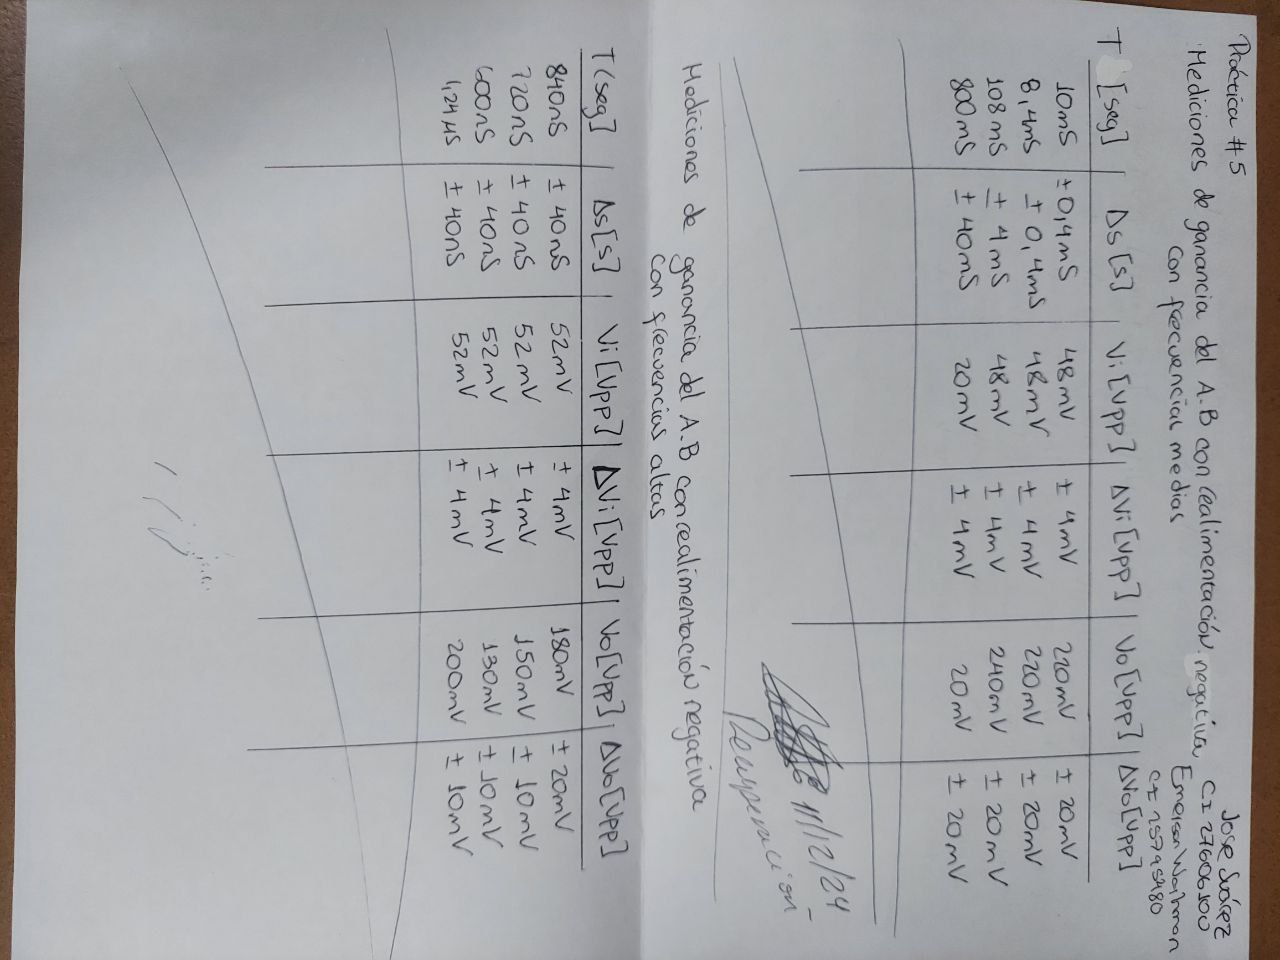
\includegraphics[width=1.0\textwidth,angle=90]{src/images/p5/p5-hoja-de-datos-2.jpg}
    \caption{Hoja de datos práctica N° 5-2}
    \label{fig:hoja-de-datos-p5-2}
\end{figure}

\begin{figure}[ht]
    \centering
    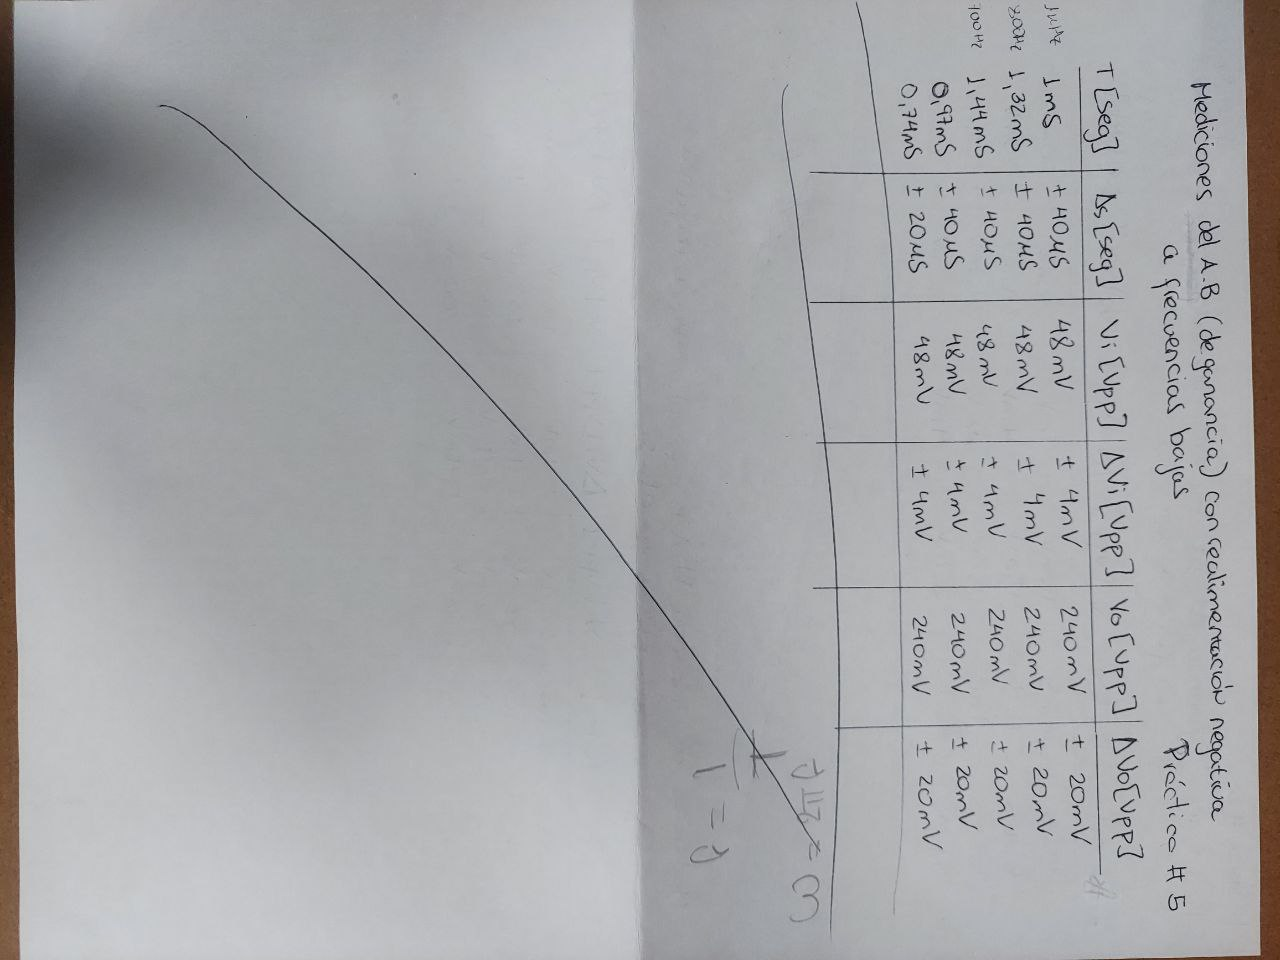
\includegraphics[width=1.0\textwidth, angle=90]{src/images/p5/p5-hoja-de-datos-3.jpg}
    \caption{Hoja de datos práctica N° 5-3}
    \label{fig:hoja-de-datos-p5-3}
\end{figure}

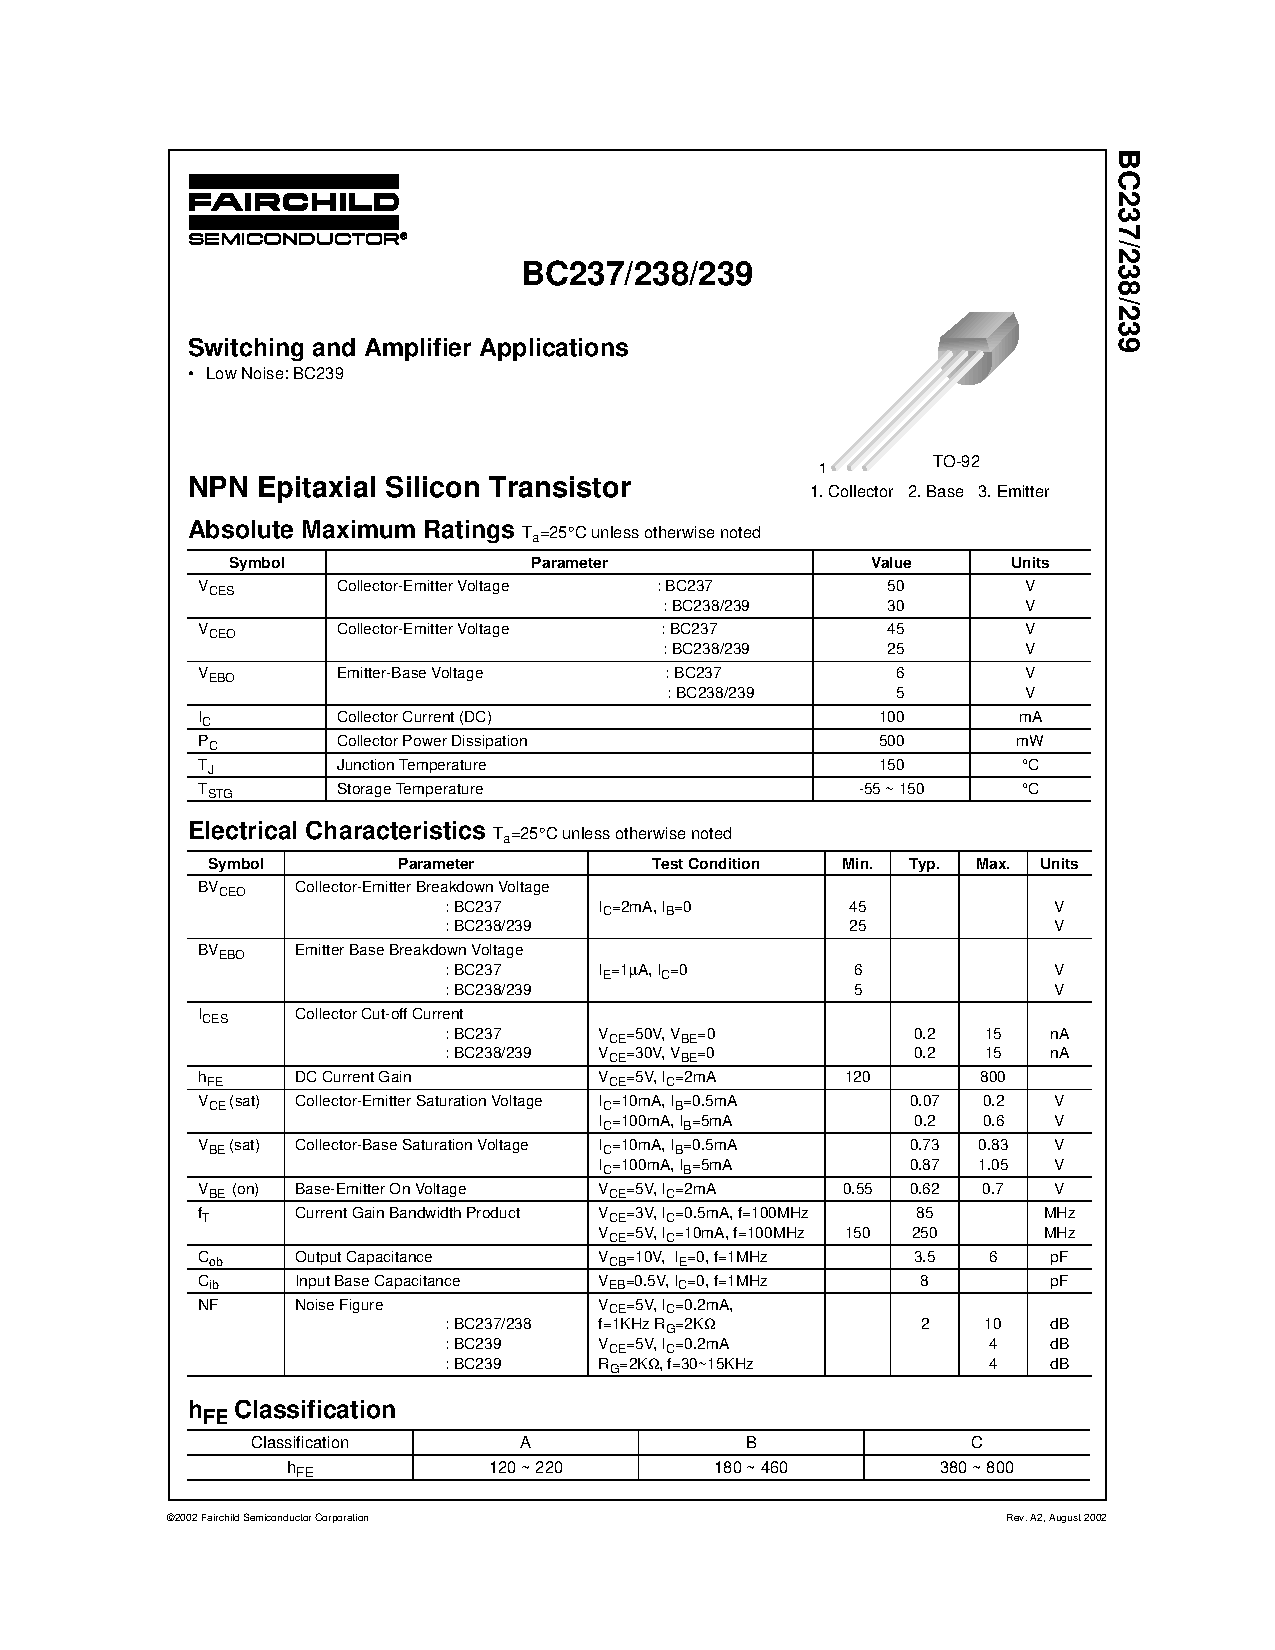
\includepdf[page=-, width=0.9\textwidth]{src/assets/BC237.pdf}
\captionof{figure}{Hoja de datos del transistor BC237}

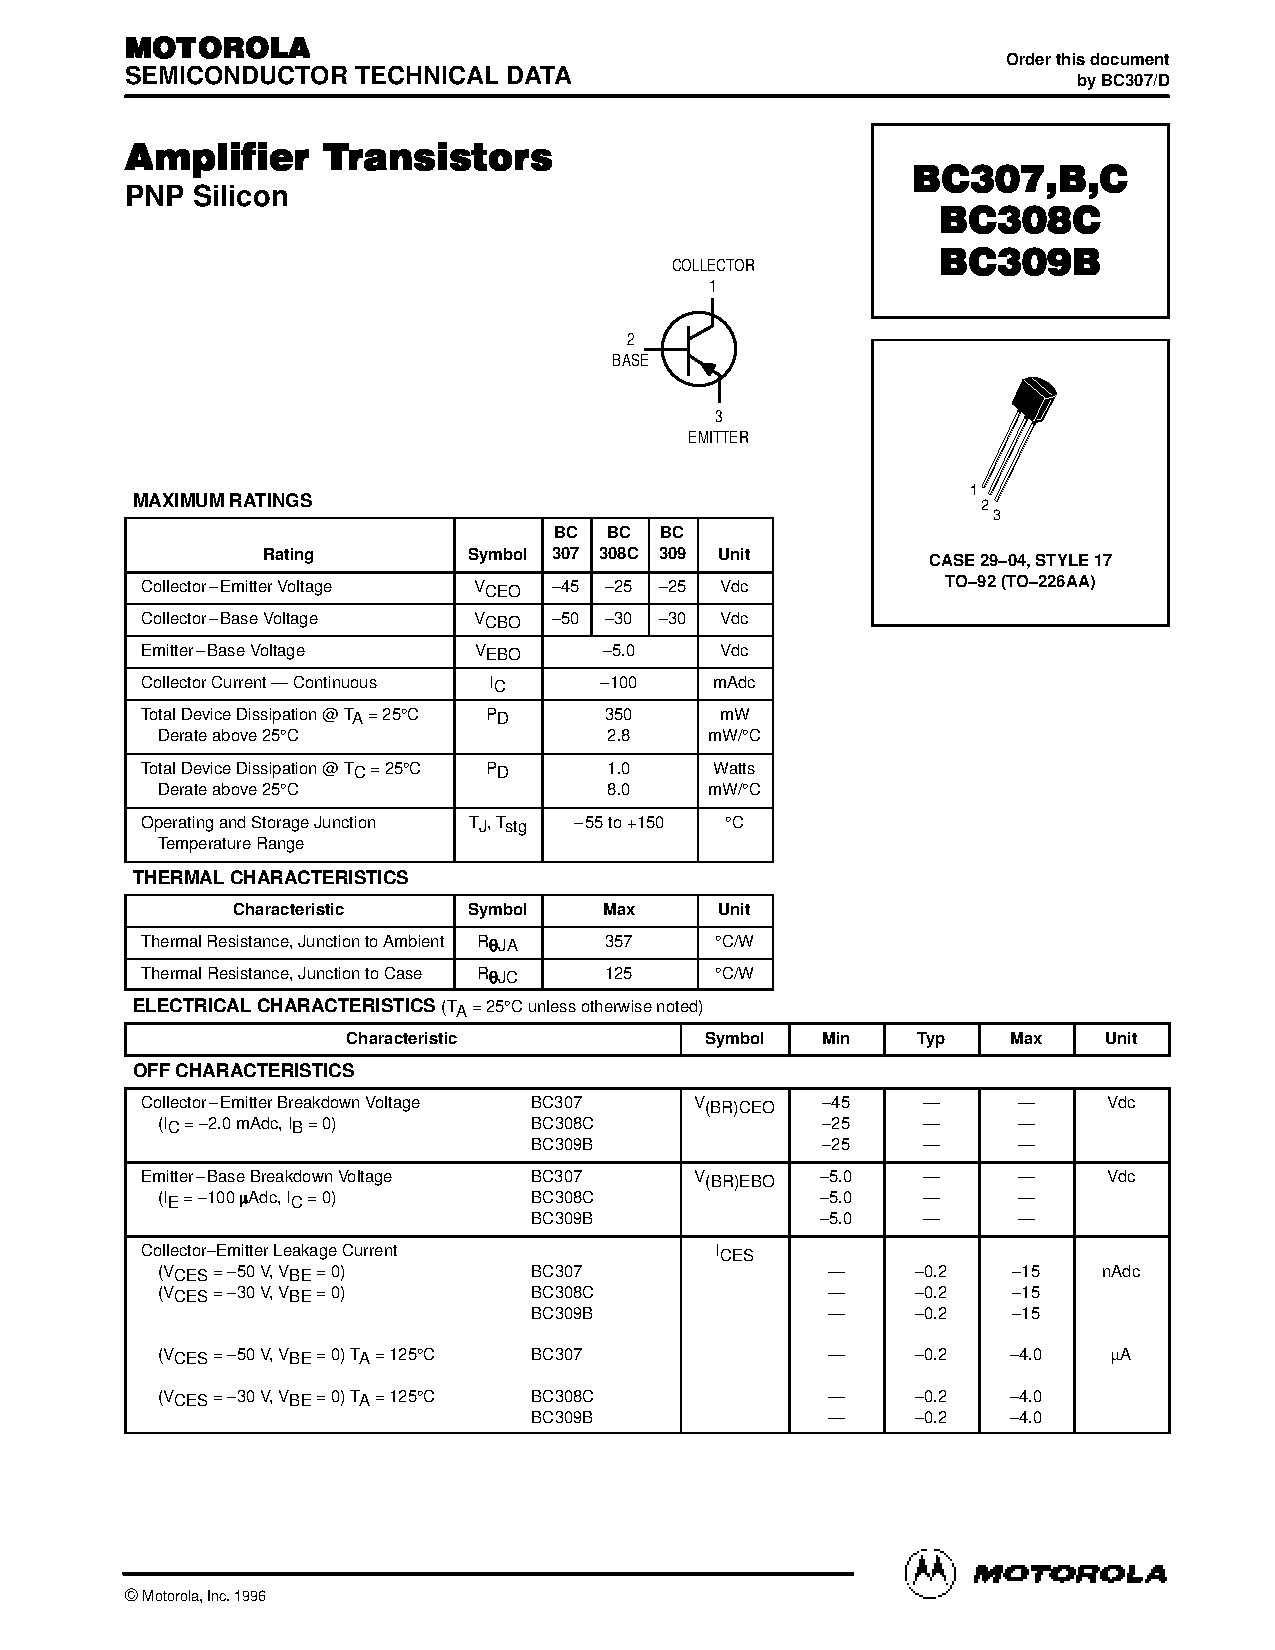
\includepdf[page=-, width=0.9\textwidth]{src/assets/bc307.pdf}
\captionof{figure}{Hoja de datos del transistor BC307}


\end{document}
